

\documentclass[10pt]{amsart}

%% PACKAGES %%%%%%%%%%%%%%%%%%%%%%%%%%%%%%

\usepackage{amsmath,amsthm,amssymb,latexsym,amstext,amsfonts,mathabx}
\usepackage[english]{babel}
\usepackage{geometry}
\usepackage{graphics,comment}
\usepackage{graphicx}
\usepackage{helvet}
\usepackage{enumitem}
\usepackage{pifont}
\usepackage{ccfonts} 
\usepackage{bbold}
\usepackage{tikz}
\usepackage{tikz-cd}
\usetikzlibrary{%
  matrix,%
  calc,%
  arrows,%
  shapes,%
  positioning%
}
\usetikzlibrary{positioning}
\usepackage{hyperref}
\usepackage{caption}
\usepackage{subfigure}

\usepackage{lineno}

\usepackage{todonotes}


\newcommand{\todoj}[2][]
{\todo[color=green, #1]{Jo\~ao: #2}}
\newcommand{\todop}[2][]
{\todo[color=green, #1]{Primo\v z: #2}}

%%%%%%%%%%%% MACROS %%%%%%%%%%%%%%%%%%%%%%%

\newtheorem{theorem}{Theorem}[section]
\newtheorem{acknowledgement}[theorem]{Acknowledgement}
\newtheorem{algorithm}[theorem]{Algorithm}
\newtheorem{axiom}[theorem]{Axiom}
\newtheorem{case}[theorem]{Case}
\newtheorem{claim}[theorem]{Claim}
\newtheorem{conclusion}[theorem]{Conclusion}
\newtheorem{condition}[theorem]{Condition}
\newtheorem{conjecture}[theorem]{Conjecture}
\newtheorem{corollary}[theorem]{Corollary}
\newtheorem{criterion}[theorem]{Criterion}
\newtheorem{definition}[theorem]{Definition}
\newtheorem{construction}[theorem]{Construction}
\newtheorem{example}[theorem]{Example}
\newtheorem{exercise}[theorem]{Exercise}
\newtheorem{lemma}[theorem]{Lemma}
\newtheorem{notation}[theorem]{Notation}
\newtheorem{problem}[theorem]{Problem}
\newtheorem{proposition}[theorem]{Proposition}
\newtheorem{remark}[theorem]{Remark}
\newtheorem{solution}[theorem]{Solution}
\newtheorem{contributions}[theorem]{Contributions}

%%%%%%%%% NOTATION %%%%%%%%%%%%%%%%%%

\newcommand{\N}{\mathbb{N}}
\newcommand{\Z}{\mathbb{Z}}
\newcommand{\R}{\mathbb{R}}
\newcommand{\A}{\mathbb{A}}
\newcommand{\B}{\mathbb{B}}
\newcommand{\Sl}{\mathbb{S}}
\newcommand{\La}{\mathbb{L}}
\newcommand{\V}{\mathbb{V}}
\newcommand{\U}{\mathbb{U}}
\newcommand{\C}{\mathbb{C}}
\newcommand{\G}{\mathbb{G}}
\newcommand{\Ff}{\mathbb{F}}
\newcommand{\I}{\mathbb{I}}
\newcommand{\F}{\mathbb{F}}
\newcommand{\W}{\mathbb{W}}
\newcommand{\X}{\mathbb{X}}
\newcommand{\Y}{\mathbb{Y}}
\newcommand{\Po}{\mathbb{P}}


\newcommand{\RR}{\mathcal R}
\def \GG{{\mathcal G}}
\def \HH{{\mathcal H}}
\def \LL{{\mathcal L}}
\def \DD{{\mathcal D}}
\def \JJ{{\mathcal J}}
\def \FF{{\mathcal F}}
\def \CC{{\mathcal C}}
\def \MM{{\mathcal M}}
\def \NN{{\mathcal N}}
\def \KK{{\mathcal K}}
\def \FF{{\mathcal F}}
\def \UU{{\mathcal U}}
\def \Pe{{\mathcal P}}
\def \SS{{\mathcal S}}
\def \AA{{\mathcal A}}
\def \BB{{\mathcal B}}
\def \VV{{\mathcal V}}
\def \II{{\mathcal I}}
\def \KK{{\mathcal K}}
\def \XX{{\mathcal X}}
\def \YY{{\mathcal Y}}
\def \EE{{\mathcal E}}


%%%%%% OPERATORS %%%%%%%%%%%%%%%%

\DeclareMathOperator{\Hom}{Hom}
\DeclareMathOperator{\dom}{dom}
\DeclareMathOperator{\im}{im}
\DeclareMathOperator{\coker}{coker}
\DeclareMathOperator*{\colim}{colim}
\DeclareMathOperator{\mmax}{max}
\DeclareMathOperator{\mmin}{min}
\DeclareMathOperator{\eq}{eq}
\DeclareMathOperator{\coeq}{coeq}
\newcommand{\Drel}{\mathbin{\mathcal D}}
\newcommand{\Rrel}{\mathbin{\mathcal R}}
\newcommand{\Lrel}{\mathbin{\mathcal L}}
\newcommand{\set}[1]{\{\,#1\,\}}
\newcommand{\x}{\mathbb{x}}
\newcommand{\Hg}{\mathrm{H}}
\newcommand{\rto}{\rightarrow}
\newcommand{\from}{\leftarrow}
\newcommand{\kk}{\mathrm{k}}
\newcommand{\meet}{\wedge}
\newcommand{\join}{\vee}
\newcommand{\bigmeet}{\bigwedge}
\newcommand{\bigjoin}{\bigvee}
\newcommand{\comp}{\circ}
\newcommand{\dsum}{\oplus}
\newcommand{\into}{\hookrightarrow}
\newcommand{\onto}{\twoheadrightarrow}

\newcommand\dfn{\textbf}


%%% FRONT %%%%%%%%%%%%%%%%%%%%%%%%%%%%%%%%%%%%%%%%%%%%%%%%%%%%%%%%

\begin{document}

\title{
\textbf{A LATTICE FOR PERSISTENCE}
}

\author{Jo\~ao Pita Costa and Primo\v z \v Skraba}

\address{In\v stitut Jo\v zef Stefan,\\
Jamova Cesta 39, 1000 Ljubljana, Slovenia.
}
\date{\today}

\maketitle

%%%%%%%%%%%%%%%  NOTES  %%%%%%%%%%%%%%%%%%%%%%%%%%%%%%%%%%%%%%%%%%%%

\begin{center}

To be submitted to the Cambridge journal of \\
\textbf{Mathematical Structures in Computer Science} \\
Editors Alex Simpson or Thierry Coquand
\medskip

\end{center}

%%% ABSTRACT %%%%%%%%%%%%%%%%%%%%%%%%%%%%%%%%%%%%%%%%%%%%%%%%%%%%%%%%


\begin{abstract} 
The intrinsic connection between lattice theory and topology is fairly well established.
For instance, the collection of open subsets of a topological subspace always forms a distributive lattice. 
Persistent homology has been one of the most prominent areas of research in computational topology in the past 20 years.
In this paper we will introduce an alternative interpretation of persistence based on the study of the order structure of its correspondent lattice. 
Its algorithmic construction leads to two operations on homology groups which describe an input diagram of spaces as a complete Heyting
algebra, which is a generalization of a Boolean algebra.  
We investigate some of the properties of this lattice, the algorithmic implications of it, and some possible applications.
\end{abstract}


%%% TABLE OF CONTENTS %%%%%%%%%%%%%%%%%%%%%%%%%%%%%%%%%%%%%%%%%%%%%%%%%%%

%\pagebreak
%
%\renewcommand{\contentsname}{Table of Contents}
%%\renewcommand{\indexname}{Index}
%
%\tableofcontents 
%
%
%
%\makeatletter
%\providecommand\@dotsep{5}
%\makeatother
%\listoftodos\relax
%
%\pagebreak
%
%


%%%%%%%%%%%%%%%%%%%%%%%%%%%%%%%%%%%%%%%%%%%%%%%%%%%%%%%%%%%%%%%%%%%
%%  MAIN MATTER                                                  %%
%%%%%%%%%%%%%%%%%%%%%%%%%%%%%%%%%%%%%%%%%%%%%%%%%%%%%%%%%%%%%%%%%%%


\linenumbers



\section*{Introduction}
\label{Introduction}

Persistent (co)homology is one of the central objects of study in applied and computational topology~\cite{Edel00}. Numerous extensions have been proposed to the original formulation including zig-zag persistence~\cite{ZigZag} and multidimensional persistence~\cite{Carl09}, whereas the original persistence looks at a filtration (i.e., an increasing sequence of spaces). Zig-zag persistence extended the theory and showed that the direction of the maps does not matter, using tools from quiver theory. In multidimensional persistence, multifiltrations are considered. In this paper, we also look at the problem of persistence in more general diagrams of spaces using tools from lattice theory. There is another key difference in this work however. Rather than try to find a decomposition of the diagram of spaces into indecomposables, we concentrate on pairs of spaces within diagrams addressing the more difficult problem of indecomposables in the sequel paper. 
Good reviews on topological data analysis are given in \cite{TD} and \cite{Zom05}, on persistent homology are given in \cite{Skr13} and \cite{Zom13}, and on zig-zag persistence are given in \cite{ZigZag}, \cite{Car09} and \cite{Oud12}.

Lattice theory is the study of order structures. The deep connections between topology and lattice theory has been known since the work of Stone~\cite{Joh86}, showing a duality between Boolean algebras and certain compact and Hausdorff topological spaces, called appropriately \emph{Stone spaces}.  
In the first section of this paper we present the basic concepts of lattice theory.
These preliminaries mostly refer to classical results on distributive lattices and Heyting algebras, and can be skipped by the reader that is familiar with the subject.
A study of lattice theory and, in general, of universal algebra, can be found in \cite{Ba40}, \cite{Sa81}, \cite{Gr71} and \cite{Gr79}.

From the latter results we discuss connections with persistent homology, and give a different perspective on several aspects of this theory. 
%In particular, we look at diagrams of spaces and retrieve general laws both based on concrete examples (like standard or zig-zag persistence) and on the interpretation of laws derived from the lattice theoretic analysis. Finally  we introduce a few algorithmic applications which we will develop further in a subsequent paper. 
In \cite{Bu14}, the authors generalize persistence modules as functors from the category of posets and order preserving maps to the category of vector spaces and linear maps. 
Such a functor assigns to each poset $\Po=(P;\leq)$ a diagram of vector spaces and linear maps with the underlying order structure of $\Po$. 
With this paper we propose the extension of the underlying poset structure to a lattice structure $\La=(L;\wedge,\vee)$ such that the following diagram commutes: 

\begin{center}
\begin{tikzpicture}[scale=.7]

  \node (c) at (0,0) {$(P;\leq)$};
  \node (d) at (0,-2.5) {$(H;\wedge,\vee)$};
  \node (b) at (2.5,0) {$Vect$};
  
\draw[arrows=-latex'] (c) -- (d) node[pos=.5,left] {};
\draw[arrows=-latex'] (d) -- (b) node[pos=.5,left] {};
\draw[arrows=-latex'](c) -- (b) node[pos=.5,left] {};

\end{tikzpicture}
\end{center}

In this sense we enrich the underlying diagram into an algebra with several nice properties, enough to constitute a Heyting algebra
In the third section we describe the order structure of our input diagram of spaces by a partial order induced by certain maps between vector spaces, and show that this order provides such a lattice structure.
We provide the construction of the meet and join operations using the natural concepts of limits and colimits of linear maps, and show that this construction stabilizes.  
We shall see that the constructed lattice is a complete Heyting algebra, one of the algebraic objects of biggest interest in topos theory.

In the last section of this paper we present the interpretation of this lattice structure in several generalizations of persistence as in multidimensional persistence or in zigzag persistence.
We also present some of the several algorithmic applications of this unification theory, including the largest injective algorithm and the section decomposition algorithm.

%%%%%%%%%%%%%%%%%%%%%%%%%%%%%%%%%%%%%%%%%%%%%%
%%%%%%%%%%%%%%%%%%%%%%%%%%%%%%%%%%%%%%%%%%%%%%



%
\section{Preliminaries}
\label{Preliminaries}

A \emph{lattice} is a partially-ordered set (or poset) expressed by $(L,\leq)$  for which all pairs of elements have an infimum and a supremum, denoted by $\wedge$ and $\vee$, respectively, commonly known as the \emph{meet} and \emph{join} operations. 
The lattice properties correspond to the minimal structure that a poset must have to be seen as an algebraic structure. 
Such algebraic structure $(L;\wedge ,\vee)$ is given by two operations $\wedge$ and $\vee$ satisfying $x\wedge (y\wedge z) = (x \wedge y)\wedge z$ and $x\vee (y\vee z) = (x \vee y)\vee z$ (\emph{associativity}); $x\wedge x = x = x\vee x$ (\emph{idempotency}); $x\wedge y=y\wedge x$ and $x\vee y=y\vee x$ (\emph{commutativity}); and $x\wedge (x\vee y)=x=x\vee (x\wedge y)$ (\emph{absorption}).
%
The equivalence between this algebraic perspective of a lattice $L$ and its ordered perspective is given by the following equivalence: for all $x,y\in L$, $x\leq y$ iff $x\wedge y=x$ iff $x\vee y=y$. 
At that stage the order and the algebraic structures hold the same information over different perspectives. 
If every subset of a lattice $L$ has a supremum and an infimum, $L$ is named a \emph{complete lattice}.
All finite lattices are complete. 
%
A partial order is named \emph{chain} (or \emph{total order}) if every pair of elements is related, that is, for all $x,y\in A$, $x\leq y$ or $y\leq x$. 
On the other hand, an \emph{antichain} is a partial order for which no two elements are related. 
%
Examples of lattices include the power set of a set ordered by subset inclusion, or the collection of all partitions of a set ordered by refinement.
%
Every lattice can be determined by a unique undirected graph for which the vertices are the lattice elements and the edges correspond to the partial order: the \emph{Hasse diagram} of the lattice. 
%
With additional constraints on the operations we get different types of lattices.  
In particular, a lattice $L$ is \emph{distributive} if, for all $x,y,z\in S$, it satisfies $x\wedge (y\vee z)=(x\wedge y)\vee (x\wedge z)$ or, equivalently, $x\vee (y\wedge z)=(x\vee y)\wedge (x\vee z)$.
While all total orders are distributive lattices, the lattice of normal subgroups of a group as well as the lattice of subspaces of a vector space are not distributive (cf. \cite{Ba40}).
A practical characterization of distributive lattices establishes that these are the lattices such that, for all $x,y,z\in L$, $x\wedge y=x\wedge z$ and $x\vee y=x\vee z$ imply 
$y=z$. This permits us a visual procedure to recognize a distributive lattice by looking at its Hasse diagram.
%
Lattice distributivity also determines the \emph{diamond isomorphism theorem} describing the isomorphism between $[a \wedge b, b]$ and $[a, a \vee b]$ using the maps $f: [a \wedge b, b] \rightarrow [a, a \vee b]$, defined by $x\mapsto x\vee a$, and $g:  [a, a\vee b]\rightarrow [a\wedge b,b]$, defined by $y\mapsto y\wedge b$. 


% Boolean algebras and Heyting algebras
%
A \emph{Boolean algebra} is a distributive lattice with a unary operation $\neg$ 
and nullary operations $0$ and $1$ such that for all elements $a\in A$, $a\vee 0 = a$ and $a\wedge 1=a$ as $a\vee \neg a = 1$ and  $a\wedge \neg a = 0$.
While the power of a set with intersection and union is a Boolean algebra, total orders are examples of distributive lattices that are not Boolean algebras in general.
%
A bounded lattice $L$ is a \emph{Heyting algebra} if, for all $a,b\in  L$ there is a greatest element $x\in L$ such that $a\wedge x\leq b$. This element is the \emph{relative pseudo-complement} of $a$ with respect to $b$ denoted by $a\Rightarrow b$. 
Examples of Heyting algebras are the open sets of a topological space, as well as all the finite nonempty total orders (that are bounded and complete). 
Furthermore, every complete distributive lattice $L$ is a Heyting algebra with the implication operation given by $x \Rightarrow y = \bigvee \set{x\in L \mid x \wedge a \leq b}$. %satisfies the \emph{infinite distributivity} identity $x\wedge \bigvee_{i\in I}y_{i}=\bigvee_{i\in I}(x\wedge y_{i})$.


\begin{contributions}
Universal algebra and lattice theory, in particular, are transversal disciplines of Mathematics and have proven to be of interest to the study of any algebraic structure. In the following sections we will describe the construction of a lattice completing a given commutative diagram of homology groups. We will show that this lattice is complete and distributive, thus constituting a complete Heyting algebra. Despite the nice algebraic properties that hold in this structure as a consequence of being such an algebra, it does not constitute a Boolean algebra.
\end{contributions} 


%%%%%%%%%%%%%%%%%%%%%%%%%%%%%%%%%%%%%%%%%%%%%%
%%%%%%%%%%%%%%%%%%%%%%%%%%%%%%%%%%%%%%%%%%%%%%



%
\section{Problem Statement}
\label{Problem Statement}


We assume a basic familiarity with algebraic topological notions such as (co)homology, simplicial complexes, filtrations, etc. 
For an overview, we recommend the references \cite{Hat00} for algebraic topology, as well as \cite{Ed10} and \cite{Zom05} for applied/computational
topology.
We motivate our constructions with the examples in the following paragraphs.

Consider persistent homology, presented in \cite{Edel00}. 
Let $\X$ be a space and $f:\X \rto \R$ a real function.  
The object of study of persistent homology is a filtration of $\X$, i.e., a monotonically non-decreasing sequence
%
\begin{equation*}
\emptyset = \X_0 \subseteq \X_1 \subseteq \X_2 \subseteq \ldots\subseteq\X_{N-1} \subseteq \X_N = \X
\end{equation*}
%
To simplify the exposition, we assume that this is a discrete finite filtration of tame spaces. Taking the homology of each of the associated chain complexes, we obtain 
%
\begin{equation*}
 \Hg_*(\X_0) \rto  \Hg_*(\X_1) \rto  \Hg_*(\X_2) \rto \ldots\rto \Hg_*(\X_{N-1}) \rto  \Hg_*(\X_N)
\end{equation*}
%
We take homology over a field $\kk$ -- therefore the resulting homology groups are vector spaces and the induced maps are linear maps. In~\cite{Edel00}, the $(i,j)-$\emph{persistent homology groups}  of the filtration are defined as
%
\begin{equation*} 
\Hg^{i,j}_*(\X) = \im (\Hg_*(\X_i) \rto   \Hg_*(\X_j))
\end{equation*}

This motivates the idea for the construction of a totally ordered lattice.
To see this, let us consider the set of the homology groups with a partial order induced by the indexes of the spaces in the filtration. We can define two lattice operations $\meet$ and $\join$ as follows:
%
\begin{itemize}
\item[] $\Hg_*(\X_i) \join \Hg_*(\X_j) = \Hg_*(X_{\max(i,j) })$
\item[] $\Hg_*(\X_i) \meet \Hg_*(\X_j) = \Hg_*(X_{\min(i,j) })$
\end{itemize}
%
With these operations we get a finite total order and, thus, a complete Heyting algebra (see this discussion in the following section). 
The definition of persistent homology groups can then be rewritten as follows:

\begin{definition}\label{rank}
For any two elements $\Hg_*(\X_i)$ and $ \Hg_*(\X_j)$, the rank of the persistent homology classes is 
\[
\im (\Hg_*(\X_i\meet\X_j) \rto \Hg_*(\X_i\join \X_j)).
\]
\end{definition}


%%%%%% MULTIDIMENSIONAL CASE %%%%%%%%%%%%%%%%%%%%%%%%%%

The case of a filtration, where a total order exists, does not have a very interesting underlying order structure. 
Let us now look at the case where we have more than one parameter. 
We define a \emph{diagram} to be a directed acyclic graph of vector spaces (vertices) and linear maps between them (edges). 
This is known as multidimensional persistence and has been studied in \cite{Carl09} and \cite{Zom09}. 
We shall start by looking at a bifiltration, i.e., a filtration on two dimensions (or parameters).
Observe that, for related elements of the filtration, these operations coincide with the ones defined above for the standard persistence case. 
However, when we consider incomparable elements, the meet and join operations are given by the rectangles they determine. 
Adjusting our definitions from above we can define the lattice operations in a natural way by setting:

\begin{itemize}
\item[] $\Hg_*(\X_{i,j}) \join \Hg_*(\X_{k,\ell}) = \Hg_*(X_{\max(i,k),\max(j,\ell) })$
\item[] $\Hg_*(\X_{i,j}) \meet \Hg_*(\X_{k,\ell}) = \Hg_*(X_{\min(i,k),\min(j,\ell) })$
\end{itemize}

Consider the bifiltration of dimensions $4\times 4$ from Figure \ref{figmulti}. The Hasse diagram of the correspondent underlying algebra is presented in Figure \ref{figmultidim}.
In that diagram, $\X_{01}\leq \X_{31}$ and clearly, $\X_{01}\meet \X_{31}=\X_{01}$ while $\X_{01}\join \X_{31}=\X_{31}$.
On the other hand, $\X_{02}$ and $\X_{11}$ are unrelated with $\X_{02}\meet \X_{11}=\X_{01}$ while $\X_{02}\join \X_{11}=\X_{12}$.
%
Note that, by the commutativity of the diagram, any two elements which have the same meet and join define the same rectangle in the bifiltration, determined by the properties in the Hasse diagrams represented in Figure \ref{figmultidim}. 
By the assumed commutativity of the diagram of spaces, any path through the rectangle has equal rank and so the map of the meet to join gives the rank invariant of Definition \ref{rank}. 

 
\begin{figure}

\subfigure[]{

\begin{tikzpicture} 
         \foreach \i in {0,...,3}{
           \foreach \j  in {0,...,3}{
             \node (p\i\j) at (\i,\j) {$\X_{\i\j}$}    ;
           }
         }
         \foreach \i [evaluate=\i as \x using int(\i+1)] in {0,...,2}{
           \foreach \j in {0,...,3}{
             \draw[->] (p\i\j) -- (p\x\j)  ;
           }
         }
     \foreach \i  in {0,...,3}{
           \foreach \j [evaluate=\j as \y using int(\j+1)] in {0,...,2}{
             \draw[->] (p\i\j) -- (p\i\y)  ;
           }
         }
\draw[thick, red] (p00) circle (0.5cm);
\draw[thick, red] (p33) circle (0.5cm);
\draw[thick,red] (p00) -- (p01.south east);

\draw[thick,red] (p01.south east) -- (p11.south east); 
\draw[thick,red] (p11.south east) -- (p12.south east); 
\draw[thick,red] (p12.south east) -- (p22.south east);
\draw[thick,red] (p22.south east) -- (p23.south east);
\draw[thick,red] (p23.south east) -- (p33);


\end{tikzpicture}
}
%
\subfigure[]{

\begin{tikzpicture} 
         \foreach \i in {0,...,3}{
           \foreach \j  in {0,...,3}{
             \node (p\i\j) at (\i,\j) {$\X_{\i\j}$}    ;
           }
         }
         \foreach \i [evaluate=\i as \x using int(\i+1)] in {0,...,2}{
           \foreach \j in {0,...,3}{
             \draw[->] (p\i\j) -- (p\x\j)  ;
           }
         }
     \foreach \i  in {0,...,3}{
           \foreach \j [evaluate=\j as \y using int(\j+1)] in {0,...,2}{
             \draw[->] (p\i\j) -- (p\i\y)  ;
           }
         }
\draw[thick, red] (p30) circle (0.5cm);
\draw[thick, red] (p03) circle (0.5cm);

\draw[thick, blue] (p00) circle (0.5cm);
\draw[thick, blue] (p33) circle (0.5cm);

\draw[red] (p00.west) -- (p03.west);
\draw[red] (p00.south) -- (p30.south);
\draw[red] (p03.north) -- (p33.north);
\draw[red] (p30.east) -- (p33.east);

\end{tikzpicture}
}
\caption{The lattice operations in the case of a bifiltration. (a) If
  the two elements are comparable, by the commutativity of the diagram
  we can choose any path to find the persistent homology groups. (b)
  If the elements are incomparable, we can find the smallest and
  largest elements where they become comparable. In both cases we
  recover the rank invariant of \cite{Carl09} }
\label{figmulti}
\end{figure}

%
\begin{figure}
%
\centering
%
\subfigure[]{%
%
     \begin{tikzpicture}[scale=.6] 
         \foreach \i  [evaluate=\i as \x using int(2*\i)] in {0,...,3}{
           \foreach \j [evaluate=\j as \y using int(2*\j)] in {0,...,3}{
             \node (p\i\j) at (\x,\y) {$\X_{\i\j}$}    ;
           }
         }
         \foreach \i [evaluate=\i as \x using int(\i+1)] in {0,...,2}{
           \foreach \j [evaluate=\j as \y using int(\j+1)]  in {0,...,2}{
             \draw[->] (p\i\j) -- (p\i\y)  ;
             \draw[->] (p\i\j) -- (p\x\j)  ;
           }
         }
%
         \foreach \j [evaluate=\j as \y using int(\j+1)]  in {0,...,2}{
           \draw[->] (p3\j) -- (p3\y)  ;
           \draw[->] (p\j3) -- (p\y3)  ;
           }
     \end{tikzpicture}
}     
% 
 \quad
% 
 \subfigure[]{%
% 
     \begin{tikzpicture}[scale=.8]

  \node (03) at (-3,1){$\X_{03}$} ;
  \node (13) at (-2,2){$\X_{13}$} ;
  \node (23) at (-1,3){$\X_{23}$} ;
  \node (33) at (0,4){$\X_{33}$} ;
  \node (32) at (1,3){$\X_{32}$} ;  
  \node (31) at (2,2){$\X_{31}$} ;
  \node (30) at (3,1){$\X_{30}$} ;  
  \node (22) at (0,2){$\X_{22}$} ;
  \node (12) at (-1,1) {$\X_{12}$} ; 
  \node (21) at (1,1){$\X_{21}$} ;
  \node (02) at (-2,0){$\X_{02}$} ;
  \node (20) at (2,0){$\X_{20}$} ;
  \node (11) at (0,0) {$\X_{11}$} ;
  \node (01) at (-1,-1){$\X_{01}$} ;
  \node (10) at (1,-1) {$\X_{10}$} ;
  \node (00) at (0,-2) {$\X_{00}$} ;
%  
  \draw (00) -- (01) -- (02) -- (03) -- (13) -- (23) -- (33) -- (32) -- (31)-- (30) -- (20) -- (10) -- (00);
  \draw (02) -- (12) -- (22) -- (32);
  \draw (01) -- (11) -- (21) -- (31);
  \draw (10) -- (11) -- (12) -- (13);      
  \draw (20) -- (21) -- (22) -- (23);  
%       
\end{tikzpicture}
}
%
\caption{The diagram of a bifiltration of dimensions $4\times 4$ (a) and the Hasse diagram of the correspondent underlying Heyting algebra (b).}
%
\label{figmultidim}       
%
\end{figure}     


\begin{figure}

\begin{center}
\begin{tikzpicture}[very thick, scale=0.8]
\node (a) at (0,0) {$\X_0$};
\node (b) at (0,2) {$\X_1$};
\node (c) at (1,3) {$\X_2$};
\node (d) at (2,0) {$\X_3$};
\node (e) at (2,2) {$\X_4$};
\node (f) at (3,-1) {$\X_5$};
\node (g) at (4,0) {$\X_6$};
\node (i) at (3,3) {$\X_7$};
\node (h) at (4,2) {$\X_8$};
\draw[->] (a) -- (b);
\draw[->] (b) -- (c);
\draw[->] (a) -- (e);
\draw[->] (d) -- (e);
\draw[->] (d) -- (b);
\draw[->] (e) -- (c);

\draw[->] (e) -- (i);
\draw[->] (h) -- (i);
\draw[->] (g) -- (h);
\draw[->] (f) -- (g);
\draw[->] (f) -- (d);

\draw[->] (d) -- (h);

\node (e1) at (1.5,-2) {\textcolor{red}{$\X_0 \wedge \X_5$}};
\draw[->,red, dashed] (e1) -- (f) ;
\draw[->,red, dashed] (e1) -- (a) ;

\node (e2) at (2,4) {\textcolor{blue}{$\X_2 \vee \X_7$}};
\draw[->,blue, dashed] (i) -- (e2) ;
\draw[->,blue, dashed] (c) -- (e2) ;

\end{tikzpicture}
\end{center}

\caption{General commutative diagrams of spaces and linear maps between them.}
\label{gendigm}
\end{figure}

Both of these cases are highly-structured. 
Consider the case of a more general diagram of homology groups in Figure \ref{gendigm}.
%
While we can embed this diagram in a multifiltration, by
augmenting the diagram with $0$ and unions of space, however the result is not very informative.
The defined lattice operations can bring a complementary knowledge to this study.
%
This is the motivation for the construction we present in this
paper. Since we deal with homology over a field, we look to analyze more
general but commutative diagrams of vector spaces. 

\begin{problem}
Given a commutative diagram of vector spaces and linear maps between
them, we  construct an order structure that completes it into a lattice, study its 
algebraic properties and develop algorithms based on this.  

\begin{center}
\begin{tikzpicture}[scale=.7]

  \node (c) at (0,0) {$(P;\leq)$};
  \node (d) at (0,-2.5) {$(H;\wedge,\vee)$};
  \node (b) at (2.5,0) {$Vect$};
  
\draw[arrows=-latex'] (c) -- (d) node[pos=.5,left] {};
\draw[arrows=-latex'] (d) -- (b) node[pos=.5,left] {};
\draw[arrows=-latex'](c) -- (b) node[pos=.5,left] {};

\end{tikzpicture}
\end{center}

\end{problem}

\begin{remark}
Quiver theory is also concerned with diagrams of vector spaces and
linear maps. However, a key difference is that the diagrams in quiver
theory are generally not required to be commutative. 
\end{remark}

\begin{remark}
We concentrate on the persistence between two elements rather than decomposition of the entire diagram. 
While we believe the constructions in this paper can aid this
decomposition, it does not immediately follow. As such, any reference
to a diagram should be understood as referring to the input collection
of vector spaces and linear maps, corresponding to the partial Hasse diagram of the underlying lattice structure, 
rather than a persistence diagram.
\end{remark}


%%%%%%%%%%%%%%%%%%%%%%%%%%%%%%%%%%%%%%%%%%%%%%
%%%%%%%%%%%%%%%%%%%%%%%%%%%%%%%%%%%%%%%%%%%%%%





%
\section{Lattice Structure}
\label{Structural Theory}


Here we introduce how to retrieve the order information from a diagram of vector spaces and linear maps, and construct the lattice operations determined by that order, where the elements are vector spaces. 
The linear maps between them will define the relations between those vector spaces and limit concepts like equalizers and coequalizers (roughly, an equalizer is a solution set of equations while a coequalizer is a generalization of a quotient by an equivalence relation) will serve us to define biggest and least elements.   

\subsection{Ordering Vector Spaces}

%%  THE POSET OF VECTOR SPACES

Consider a diagram of vector spaces and linear maps and assume one unique component.
The underlying ordered structure is a poset defined as follows: 

\begin{definition}
For all vector spaces $A$ and $B$ of a given diagram $\DD$,
\[
A\leq B\text{  if there exists a linear map  }f:A\rightarrow B.
\]
\end{definition}
%
The partial order $\leq $ is, thus, the set of ordered pairs correspondent to the linear maps in the commutative diagram of spaces given as input.
The identity map ensures the reflexivity of the relation: for all vector spaces $A$ the identity map $id_A$ provides the endorelation $\lefttorightarrow A$.
Transitivity is given by the fact that the composition of linear maps is a linear map and by the assumption that all diagrams are commutative. 
Antisymmetry is given by the fact that $A\leftrightarrows B$ implies $A\leftrightsquigarrow B$, that is, $A$ and $B$ are equal up to isomorphism: 
in detail, having the identity morphisms and usual composition of linear maps, the existence of linear maps $f:A\rightarrow B$ and $g:B\rightarrow A$ imply that $g\circ f=id_{A}$ and that $f\circ g=id_{B}$, as required.
%
This partial order does not yet have to constitute a lattice but will be completed into one, due to the following constructions. 
The extension of the partial order $\leq$ will be noted by the same symbol, being a part of that bigger partial order.

\begin{remark}
We consider the object under study to be a commutative diagram of vector spaces and linear maps. As vector spaces are determined up to isomorphism by rank, the equivalence deserves some additional comments. As described above, the reverse maps exist in the case of isomorphisms. This further ensures that the poset structure is well-defined since we cannot arbitrarily reverse the direction of the arrows (as is often the case in representation theory, where the direction of arrows often does not matter). 
If we were to reverse an arrow with a non-unique (but equal rank) map, it is clear that the composition will not commute with identity unless the map is an isomorphism. 
Likewise,  for equivalence we not only require the vector spaces to be isomorphic (of the same rank) but also that there exists a composition of maps in the diagram (possibly including inverses) for which an isomorphism exists. 
Note that this does not imply that all the maps must be isomorphisms. 
\end{remark}







\subsection{The Lattice Operations}
% 
% 
%% %%%%%%%%%%%% DEFINITION OF THE LATTICE OPERATIONS %%%%%%%%%%%%%
%
%
In the following paragraphs we will describe the construction of the operations $\wedge $ and $\vee$ over a given diagram $\DD$ of vector spaces and linear maps.
The construction of these lattice operations is based on the concept of direct sum, and the categorical concepts of \emph{limit} and \emph{colimit} (and, in particular, on generalized notions of \emph{equalizer} and \emph{coequalizer}).

\begin{definition}
A vector space is a \emph{source} if it is no codomain of any map, and dually it is a \emph{target} if it is no domain of any map (corresponding to the categorical concepts of \emph{initial element} and \emph{terminal element}, respectively. 
Moreover, we call \emph{common source} of a collection of spaces $D_i$ in the given diagram $\DD$, to a space $D\in \DD$ mapping in $\DD$ to each of the spaces $D_i$.
Dually, we call \emph{common target} of the collection $D_i$ to a space $D\in \DD$ such that each $D_i$ maps to $D$.
\end{definition}

\begin{remark}\label{exist}
Given vector spaces $X$, $Y$, $Z$ and $W$ in a diagram $\DD$,

\begin{itemize}
\item[(i)] if $Z$ is a common target of $X$ and $Y$ then $Z$ is a target of $X\oplus Y$;
\item[(ii)] if $W$ is a common source of $X$ and $Y$ then $W$ is a source of $X\oplus Y$.
\end{itemize}
%
While $(i)$ follows from the fact that the direct sum is the coproduct in the category of vector spaces and linear maps, to see $(ii)$ consider the inclusion maps $i_{X}:X\rightarrow X\oplus Y$ and $i_{Y}:Y\rightarrow X\oplus Y$. To see $(ii)$ consider the inclusion maps $i_{X}:X\rightarrow X\oplus Y$ and $i_{Y}:Y\rightarrow X\oplus Y$.
Due to the hypothesis, there exist maps $f:W\rightarrow X$ and $g:W\rightarrow Y$. Thus, the compositions $i_{X}\circ f$ and $i_{Y}\circ g$ ensure the inequality $W\leq X\oplus Y$.  
%
Moreover, 
\begin{itemize}
\item[(iii)] if $Z$ is a common target of $X$ and $Y$, the limit of all linear maps from $X$ and $Y$ to $Z$ is a subalgebra of $X\oplus Y$;
\item[(iv)] if $W$ is a common source of $X$ and $Y$, the colimit of all linear maps from $W$ to $X$ and $Y$ is a quotient algebra of $X\oplus Y$.
\end{itemize}
both of them constituting vector spaces. 
%
\end{remark}


\begin{definition}
  Given a diagram of vector spaces and linear maps $\DD$, 
  and arbitrary vector spaces $X$ and $Y$ in $\DD$
  we call \dfn{meet} of spaces $X, Y$ to the limit in $\DD$ 
  of all linear maps from $X\oplus Y$ to common targets of $X$ and $Y$, i.e., 
    \[
  X\meet Y = \lim\set{X\to Z\from Y : 
    Z \text{ common target of $X$ and $Y$}}
  \]
  Dually, we call \dfn{join} of spaces $X, Y$ to the colimit in $\DD$  
  of all linear maps from common sources of $X$ and $Y$ to $X \oplus Y$, i.e., 
    \[
  X\join Y = \colim\set{X\from Z\to Y : 
    Z \text{ common source of $X$ and $Y$}}
  \] 
\end{definition}








%%%%%%%%%%  WELL DEFINED OPERATIONS %%%%%%%%%%%%%%%%%%%%%%


\begin{theorem}\label{existence1} 
The operations $\wedge$ and $\vee $ are well defined.
\end{theorem}

\begin{proof}
Let $A$ and $B$ be vector spaces. 
There always exist vector spaces $C$ and $D$ such that $D\leq A,B\leq C$: the vector space $C$ can at least be $A\oplus B$ with the inclusion maps $A, B \rightrightarrows A\oplus B$; the existence of $D$ is proved similarly due to always having $\set{0}\leq A,B$.
Take $C$ to be a vector space such that $A,B\leq C$ (its existence is guaranteed by Remark \ref{exist}). 
Then, $A\oplus B\leq C$. 
Construct $A\wedge B$ as the limit of all maps $A\oplus B\rightarrow C$ as above. 
The existence of $A\vee B$ is proved similarly as we always have $\set{0}\leq A,B$.
With this we prove that the operations $\wedge$ and $\vee $ are well defined.
\end{proof}









%%%%%%%%%%%%%% STABILIZATION %%%%%%%%%%%%%%%%%%%%%%%%%%



\begin{theorem}\label{stabilize}
Given vector spaces $A$ and $B$, the construction of $A\wedge B$ and $A\vee B$ stabilizes.
\end{theorem}

\begin{proof}
In the following proof we will show that the skew lattice construction stabilizes, i.e., whenever we are given vector spaces $A$ and $B$ and
\begin{itemize}
\item[(1)] we first construct $A\wedge B$ from $A,B\leq A\oplus B$, 
\item[(2)] then we construct $A\vee B$ from $A\wedge B\leq A,B$, 
\item[(3)] then we again construct $(A\wedge B)'$ from $A,B\leq A\vee B$,
\end{itemize}

\noindent we can ensure that $(A\wedge B)'=A\wedge B$.
The dual result follows analogously.

\textbf{Case 1: Sources.}
In this case, we assume that the elements are two sources and that there exists an element above both of them. We denote the elements $A$, $B$ and $C$, respectively. We are then able to define $M=A\meet B$ that is constituted by elements $(a,b)$ of $A\oplus B$ such that $(f,0)(a,b) = (g,0)(a,b)$, where $f$ and $g$ map to $C$. Since there is now an element below $A$ and $B$, we can define  $J=A\join B$ as all the quotient space of $A\oplus B$. Define $M\rto A\oplus B$  where the map is $(k,\ell)$. Therefore we now have $A\oplus B \rto A\oplus B /\langle (k(x), \ell(x)) \mid x\in M \rangle$. Call these maps $v$ and $w$. What remains to show is that the elements which satisfy  $(v,0)(a,b) = (0,w)(a,b)$ are the same as above. Now if $(f,0)(a,b) = (g,0)(a,b)\neq (0,0)$, by commutivity and universality,  $(v,0)(a,b) = (0,w)(a,b)\neq (0,0)$. However, if $(f,0)(a,b) = (g,0)(a,b) =  (0,0)$, then there exists an element $m \in M$ such that $m\mapsto (a,b)$ which implies that $(v,0)(a,b) = (0,w)(a,b)$, since this is precisely the relation in the definition.  Since $M$ can only get smaller with additional constraints, it follows that the resulting $M$ has stabilized.

\textbf{Case 2: Targets.}
In this case, we assume that the elements are two sources and that there exists an element below them. We denote the elements $A$, $B$ and $C$ respectively. We define  $J=A\join B$, constituted by the quotient  $A\oplus B / \langle (f(x), g(x))\mid x\in C \rangle$. Denote this map $(k,\ell)$. Based on this we define the $M=A\meet B$ as the subspace such that $(k,0)(a,b) =(0,\ell)(a,b)$. Denote the map from this space to the direct sum as $(v,w)$. Now we need to show $A\oplus B /\langle (f(c), g(c))\mid c\in C \rangle = A\oplus B /\langle (v(m), w(m))\mid m\in M \rangle$. By universality  it follows that there exists an $m \in M $ such that $c \mapsto m$ and hence $f(c) = v(m)$ and $g(c) = w(m)$. It follows that $f(c) \theta g(c)$ is equivalent to  $v(m) \theta w(m)$. 
%
If we do not want to use universality, if $(f,g)(c)\neq (0,0)$, there must be an element in $J$ such that $k((f(c)) = \ell(g(c))=j$. Hence we conclude that there is an element $c\mapsto m$. If $(f,g)(c) =  (x,0)$, then  by the quotient $k(f(c)) = 0 $ and again there must be an element $m \mapsto (x,0)$.  Finally if $(f,g)(c) =  (0,0)$, there is no element other than 0 such that $k(f(c)) = \ell(g(c))$ and hence $c \mapsto (0,0) \in M$. 

\end{proof}




%%%%%%%%%%%%%%%%%% THE LATTICE PROOF %%%%%%%%%%%%%%%%%%%%%

In the following result we will show that the elements of a commutative diagram of
vector spaces together with the operations $\vee $ and $\wedge $ defined above determine a lattice.  
We will refer to it as the \emph{persistence lattice} of a given diagram of vector spaces and linear maps, 
i.e., the completion of that diagram into a lattice structure using the lattice operations $\vee $ and $\wedge $.

\begin{theorem}
Let $\DD$ be a diagram of spaces and maps between them. 
Consider the partially ordered set $\Pe=(\DD^*;\leq)$, with the operations $\vee $ and $\wedge $ defined as above, 
where $^*$ is the closure of $P$ relative to these operations.
Then $\Pe$ constitutes a lattice.
\end{theorem}

\begin{proof}
Let us see that $A\wedge B$ is the biggest lower bound of the set $\set{A,B}$.
Due to Remark \ref{exist} we need only to see that given another vector space $D$ such that $D\leq A,B$, then there exists a linear map from $D$ to $A\wedge B$, i.e., $D \leq A\wedge B$. 
Let us consider the following diagram:

\begin{center}
\begin{tikzpicture}

\node (o) at (1,3) {$A\oplus B$};
\node (a) at (0,2) {$A$};
\node (b) at (2,2) {$B$};
\node (d) at (1,-1) {$D$};
\node (ab) at (1,0.5) {$A\wedge B$};

\draw[arrows=-latex'] (a) -- (o) node[pos=.5,right] {};
\draw[arrows=-latex'] (b) -- (o) node[pos=.5,right] {}; 
\draw[->, bend left] (d) to node {} (a) ;
\draw[->, bend right] (d) to node {} (b) ;
%\draw[arrows=-latex', bend left] (d) -- (a) node[pos=.5,above] {};
%\draw[arrows=-latex', bend right](d) -- (b) node[pos=.5,left] {};
\draw[arrows=-latex', dashed] (ab) -- (a) node[pos=.5,right] {};
\draw[arrows=-latex', dashed] (ab) -- (b) node[pos=.5,right] {};
\draw[arrows=-latex', dashed,blue] (d) -- (ab) node[pos=.5,right] {};

\end{tikzpicture}  
\end{center}  

The compositions of either with the maps from $A$ and $B$ to some common target $C$ ($A\oplus B$, for instance) commute by assumption.
Due to the construction of $A\wedge B$ as a limit, we get that $D\leq A\wedge B$ by universality.
Hence, $A\wedge B$ is the greatest lower bound (the biggest subalgebra) regarding all the other subalgebras of $A\oplus B$ that are maps from $A\oplus B$ to the vector spaces above both $A$ and $B$.
%
The proof that $A\vee B$ is the least upper bound (the finest partition) of the set $\set{A,B}$ is analogous and derives from the universality of its construction as a colimit.
\end{proof}






%%%%%%%%% COMPLETION %%%%%%%%%%%%%%%%%%%%%%%%%%%%%%%


\begin{theorem}\label{complete}
Persistence lattices are complete, i.e., both of the lattice operations extend to arbitrary
joins $\bigjoin_i D_i$ and meets $\bigmeet_i D_i$ (note that both
$\bigjoin_i D_i$ and $\bigmeet_i D_i$ might not be in $\DD$).
\end{theorem}

\begin{proof}
Consider an arbitrary family $\set{X_i}_{i\in I}$ of vector spaces of the underlying persistence lattice $\Pe$ of a given diagram $\DD$. 
According to our definition of $\meet$, the $\bigmeet$ of spaces $X_i$ is the limit in $\Pe$ of all linear maps from $\oplus_{i\in I} X$ to common targets of $X_i$, i.e., 
    \[
  \bigmeet_{i\in I} X_i = \lim\set{X_i\to Z :  Z \text{ common target of $X_i$}}
  \]
Dually, the $\bigjoin$ of spaces $X_i$ is the colimit in $\Pe$ of all linear maps from common sources of $X_i$ to $\oplus_{i\in I} X$ , i.e., 
    \[
  \bigjoin_{i\in I} X_i = \colim\set{X_i\from Z :  Z \text{ common source of $X_i$}}
  \] 
%
\end{proof}

\begin{remark}
Completeness is a very important property in the study of ordered structures.
The open sets of a topological space, ordered by inclusion, are examples of such structures where $\vee$ is given by the union of open sets and $\wedge$ by the interior of the intersection. 
In the last section we will see an algorithm application for this particular lattice property. 
We will refer to it as \emph{the largest injective} by then.  
\end{remark}


%%%%%%%%%%%%%%%%%%%%%%%%%%%%%%%%%%%%%%%%%
%%%%%%%%%%%%%%%%%%%%%%%%%%%%%%%%%%%%%%%%%
 
 
 
 
 
 

\subsection{Structural Consequences}

In the following we describe some of the most relevant characteristics of the lattice that we have described in the earlier section.
We shall see that, besides the algebraic properties due to its lattice nature, it is also modular and distributive. 
%
%%%%%%%%%%%%%%% BASIC LATTICE PROPERTIES %%%%%%%%%%%%%%%%%%%%
%

\begin{remark}
Let us first have a look at the properties of the operations $\wedge$ and $\vee$ of the persistence lattice $\HH$ constructed above over an input poset. 
The identity map implies that $A\wedge A=A$ and $A\vee A=A$. 
This algebraic property follows from the order structure of the correspondent persistence lattice. 
The equivalence between the algebraic structure and the order structure of the underlying algebra ensures that a linear map $f:A\rightarrow B$ exists iff $A=A\wedge B$ iff $A\vee B=B$. 
Moreover, the following lattice identities hold:
\[
A\wedge (A\vee B)=A=A\vee (A\wedge B)=A.
\]

%\begin{itemize}
%\item[(i)] $(A\wedge B)\wedge C=A\wedge (B\wedge C)$ and $(A\vee B)\vee C=A\vee (B\vee C)$;
%\item[(ii)] $A\wedge B=B\wedge A$ and $A\vee B=B\vee A$;
%\item[(iii)] $A\wedge (A\vee B)=A$ and $A\vee (A\wedge B)=A$.
%\end{itemize}

\end{remark}


%%%%%%%%%%%%%%%%%%%%%%%%%%%%%%%%

The following result will enlighten this theory with a nice relation between the lattice operations and the direct sum. This property is not frequently used in the study of lattice properties but will permit us to show the distributivity of a persistence lattice in the next paragraphs.

\begin{theorem}\label{ses}
Let $A$ and $B$ be vector spaces. Then, \[
A\wedge B\rightarrow A\oplus B\rightarrow A\vee B \text{  is a short exact sequence.}
\]
\end{theorem}

\begin{proof}
First observe that the limit map $f:A\wedge B\rightarrow A\oplus B$ is injective and the colimit map $g:A\oplus B\rightarrow A\vee B$ is surjective (cf. \cite{La98}).
We thus need to show that $\im f=\ker g$ to prove the isomorphism 
\[
A\vee B\cong A\oplus B/f(A\wedge B).
\]

If $y\in \im f$ then there exists $x\in A\wedge B$ mapping to $y$ such that $g_{i}(x)=g_{j}(x)$ for all $g_{k}:A\oplus B\rightarrow A\vee B$ and thus $y\in \ker g$.
On the other hand, if $x\in \ker g$, then $g_{|A}(x_{|A}) = g_{|B}(x_{|B})$ implying there exists an element in $x\in A\wedge B$ which maps to $y$.

\end{proof}



%%%%%%%%%% Distributivity %%%%%%%%%%%%%%%%%%%%%%%%%%%%%%%%%%%%%%

\begin{theorem}\label{distributive}
Persistence lattices are distributive.
\end{theorem}

\begin{proof}
Let $A$, $B$ and $X$ be vector spaces such that $X\vee A=X\vee B$ and $X\wedge A=X\wedge B$ in order to show that $A\cong B$. 
Consider the following commutative diagram of spaces:

\begin{center}
\begin{tikzpicture}[scale=.7]

  \node (c) at (0,2.5) {$ X\vee A=X\vee B$};
  \node (d) at (0,-2.5) {$X\wedge A=X\wedge B$};
  \node (a) at (-2.5,0) {$A$};
  \node (b) at (2.5,0) {$X$};
  \node (x) at (0,0) {$B$};
  
\draw[arrows=-latex'] (a) -- (c) node[pos=.5,left] {$f$};
\draw[arrows=-latex'] (d) -- (a) node[pos=.5,left] {$g$};
\draw[arrows=-latex'](x) -- (c) node[pos=.5,left] {$u$};
\draw[arrows=-latex'] (d) -- (b) node[pos=.5,right] {$t$};
\draw[arrows=-latex'](d) -- (x) node[pos=.5,left] {$v$};
\draw[arrows=-latex'](b) -- (c) node[pos=.5,right] {$s$};

\end{tikzpicture}
\end{center}

\noindent
The result will follow from the definition of distributivity for the lattice operations, the Five Lemma
and exactness of the sequence (cf. Theorem \ref{ses})
\begin{equation*}
0\rightarrow Y\wedge Z \xrightarrow{f} Y\oplus Z \xrightarrow{g} Y\vee Z \rightarrow 0 
\end{equation*}
Consider the the following diagram
\begin{center}
\begin{tikzcd}
0 \arrow{r} \arrow[leftrightarrow]{d}{\cong} & A\wedge X \arrow{r} \arrow[leftrightarrow]{d}{\cong} & A\oplus X \arrow{r} &A\vee X \arrow{r} \arrow[leftrightarrow]{d}{\cong}&0 \arrow[leftrightarrow]{d}{\cong} \\
0 \arrow{r} & B\wedge X \arrow{r} & B\oplus X \arrow{r} &B\vee X \arrow{r} &0 
\end{tikzcd}
\end{center}
%
The first and last isomorphism are trivial, while the other isomorphisms follow by assumption. 
The existence of the linear map $f: A\oplus B \rightarrow B\oplus X$ is ensured by the fact that we are dealing with vector spaces, assuming the commutativity of the diagram. %providing us with the modularity of the lattice.
Therefore, by the Five Lemma, we conclude that $A\oplus X \cong B\oplus X$ and hence $A\cong B$, concluding the proof.

\end{proof}

The distributive property is of great interest in the study of order structures. With it we are able to retrieve a rich structure satisfying many interesting identities. The next result follows directly from the distributivity of persistence lattices.

\begin{corollary}
The persistence lattice intervals $[A \wedge B, B]$ and $[A, A \vee B]$ are isomorphic due to the maps $f: [A\wedge B,B] \rightarrow [A,A\vee B]$, defined by $X\mapsto X\vee A$, and $g:  [A, A\vee B] \rightarrow [A\wedge B,B]$, defined by $Y\mapsto Y\wedge B$.
\end{corollary}

%\begin{remark}
%Due to Dilworth's results on poset decompositions, there exists an antichain of vector spaces $S$ and a partition of the order in $A$ into a family $F$ of total orders of vector spaces such that the number of total orders in the partition equals the cardinality of $S$ and, thus, $S$ is the largest antichain in the order, and $F$ must be the smallest family of total orders into which the order can be partitioned. 
%Dually, the size of the largest total order of vector spaces in a finite poset of vector spaces as such equals the smallest number of antichains of vector spaces into which the order may be partitioned.
%\end{remark}


%%%%%%%%%%%% Discrete, Bounded and Finiteness %%%%%%%%%%%%%%%%%%%%%%%%%%

\begin{theorem}\label{discrete}
Persistence lattices are discrete, finite and bounded.
\end{theorem}

\begin{proof}
In the following we will give an upper bound for the number of elements of a persistence lattice of a given diagram of spaces.
The finiteness of the lattice implies that it is discrete and complete. Thus, it follows that it is a bounded lattice. 
%
Indeed, an upper bound for the number of elements of the persistence lattice correspondent to a diagram with $\mid V\mid =n$ is given by 
\[
\sum_{i} \binom{n}{i} 2^{i-1}\leq 2^{n}.2^{n}=2^{2n}.
\]
To see the above bound consider a string of $V_i$'s. Since the
operations are commutative and associative, we will need to only
consider all combinations of nodes which are included in the string.
To get an element of the lattice, we must also consider the two operations. For a string of length of $m$, this implies $m-1$ operations. Since we have two operations this implies there are $2^{(m-1)}$ operations on the string. Since $m<n$, we can bound the sum by $2^{2n}$, implying that we add a  finite number of elements. 
\end{proof}

\begin{remark}
This is a very loose bound intended only to illustrate finiteness. In practice, there will be far fewer elements due to distributivity and even fewer elements of interest.  
\end{remark}


%%%%%%%%%%%%%% complete Heyting algebra %%%%%%%%%%%%%%%%%%%%%%%%%% 

%Recall that nonempty finite distributive lattices are bounded and complete, thus forming Heyting algebras. 
%Though, Theorems \ref{distributive}, \ref{complete} and \ref{discrete} imply the next result.

\begin{theorem}
Persistence lattices constitute complete Heyting algebras.
Hence, the following identity holds: 
%\[
%A\wedge \bigvee_{i\in I}B_{i}=\bigvee_{i\in I}(A\wedge B_{i})
%\]
\end{theorem}

\begin{proof}
Recall that nonempty finite distributive lattices are bounded and complete, thus forming Heyting algebras. 
Hence, this result follows from Theorems \ref{distributive}, \ref{complete} and \ref{discrete}.
\end{proof}

\begin{remark}
Whenever $A$ and $B$ are vector spaces in a diagram, there exists a vector space $X$ that is maximal in the sense of $X\wedge A\leq B$, i.e., the implication operation is given by the colimit 
\[
A \Rightarrow B=\bigvee \set{X_i\in L \mid \bigoplus_i (X_i\wedge A) \rightarrow B}.
\]
Observe that the case of standard persistence we have that 
\[
A\Rightarrow B = \begin{cases} B, & \mbox{if } B\leq A\\ 1, & \mbox{if } A\leq B \end{cases}.
\]
The study of the interpretation of the implication operation in the framework of other general models of persistence, as zig-zag or multidimensional persistence, is a matter of further research.
\end{remark}

\begin{remark}
Persistence lattices $\Pe$ are not Boolean algebras. 
To see this just consider the standard persistence case that is represented by a total order, or the total order $\set{C,B,D}$ in the above bifiltration and observe that there is no $X\in L$ such that $B\wedge X=D$ and $B\vee X=C$. Hence, $B$ also doesn't have a complement in $\Pe$.
\end{remark}

\begin{remark}
The results of this section permit us to discuss several directions of future work that can contribute with further information on the order and algebraic properties of this structure and motivate the construction of new algorithms. 
A \emph{topos} is essentially a category that ''behaves" like a category of sheaves of sets on a topological space, while \emph{sheaves} of sets are functors designed to track locally defined data attached to the open sets of a topological space and transpose it to a global perspective using a certain ''gluing property". 
Topos theory has important applications in algebraic geometry and logic (cf. \cite{Lang} and \cite{Joh86}), and has recently been used to construct the foundations of quantum theory (cf. \cite{Is08}).
The category of sheaves on a Heyting algebra is a topos (cf. \cite{CatCS}).
Whenever skew lattices, a noncommutative variation of lattices, satisfy a certain distributivity, they constitute sheaves over distributive lattices (and over Heyting algebras in particular (cf. \cite{Ba13}). 
The study of such algebras, developed by the second author of this paper in \cite{Le13}, might be of great interest to the research on the properties of persistence lattices and their interpretation in the framework of persistent homology.
Furthermore, complete Heyting algebras are of great importance to study of frames and locales that form the foundation of pointless topology, leading to the categorification of some ideas of general topology (cf. \cite{Joh86}).
\end{remark}


\begin{remark}
A natural and well studied relationship between lattice theory and topology is described by the duality theory \cite{Da02}.  
These dualities are of great interest to the study of algebraic and topological problems taking advantage of the categorical equivalence between respective structures (cf. \cite{Fa96}).
In the case of complete Heyting algebras, the Esakia duality permits the correspondence of such algebras to dual spaces, called \emph{Esakia spaces} that are compact topological spaces equipped with a partial order, satisfying a certain separation property that will imply them to be Hausdorff and zero dimensional (cf. \cite{Be06}).  
These spaces are a particular case of \emph{Priestley spaces} that are homeomorphic to the spectrum of a ring (cf.\cite{Be10}). 
We are interested in the study of such topological spaces and correspondent ring. 
\end{remark}




%%%%%%%%%%%%%%%%%%%%%%%%%%%%%%%%%%%%%%%%%%%%%%
%%%%%%%%%%%%%%%%%%%%%%%%%%%%%%%%%%%%%%%%%%%%%%

%
\section{Algorithms and Applications}
\label{Algorithms and Applications}

We now give some interpretations of both the order structure and the algebraic structure of the lattice in the framework of persistent homology. 

\subsection{Interpretations Under Persistence}

We saw that in the case of standard persistence, we have a total order where $A$ and $B$ are related and thus $(L1)$ tells us that, $\X_{m}\wedge \X_{n}=\X_{m}$, the domain of the map $f$ connecting $\X_{m}$ and $\X_{n}$, while $\X_{m}\vee \X_{n}=\X_{n}$, its codomain.
%
On the other hand, to analyze the multidimensional case we saw that using  
\[
\X_{n,m}\wedge \X_{p,q}=\X_{\min\set{n,p},\max\set{m,q}} \text{  andÊ } \X_{n,m}\vee \X_{p,q}=\X_{\max\set{n,p},\min\set{m,q}}.
\] 
for the meet and join respectively we recover the rank invariant. 
We will return to the bifiltration case but first discuss its connections with zig-zag persistence. 
%
In the case of zig-zag persistence, we get the following diagram:

\begin{center}
\begin{tikzpicture}
\node (a) at (0,0 ) {$\Hg(\X_0)$};
\node (b) at (2,0 ) {$\Hg(\X_2)$};
\node (c) at (4,0 ) {$\Hg(\X_4)$};
\node (d) at (6,0 ) {$\Hg(\X_6)$};
\node (e) at (8,0 ) {$\Hg(\X_8)$};
\node (w) at (1,1 ) {$\Hg(\X_1)$};
\node (x) at (3,1 ) {$\Hg(\X_3)$};
\node (y) at (5,1 ) {$\Hg(\X_5)$};
\node (z) at (7,1 ) {$\Hg(\X_7)$};
\draw[->] (a) -- (w);
\draw[->] (b) -- (w);
\draw[->] (b) -- (x);
\draw[->] (c) -- (x);
\draw[->] (c) -- (y);
\draw[->] (d) -- (y);
\draw[->] (d) -- (z);
\draw[->] (e) -- (z);
\end{tikzpicture}
\end{center}
%
Without loss of generality, if we assume that we have an alternating zig-zag as above, we see that we have a partial order: the odds are strictly greater than the even indexed spaces.  This is not an interesting partial order as most elements are incomparable. 
%
In ~\cite{Car09} and~\cite{Be12} it was noted that using unions and relative homology, the above could be extended to a case where all elements become comparable with possible dimension shifts. 
The resulting zig-zag can be extended into a M\" obius strip through exact squares. By exactness any two elements can be compared by considering unions and relative homologies as shown in Figure~\ref{fig:zz}. 

\begin{figure}[ht]
\begin{center}
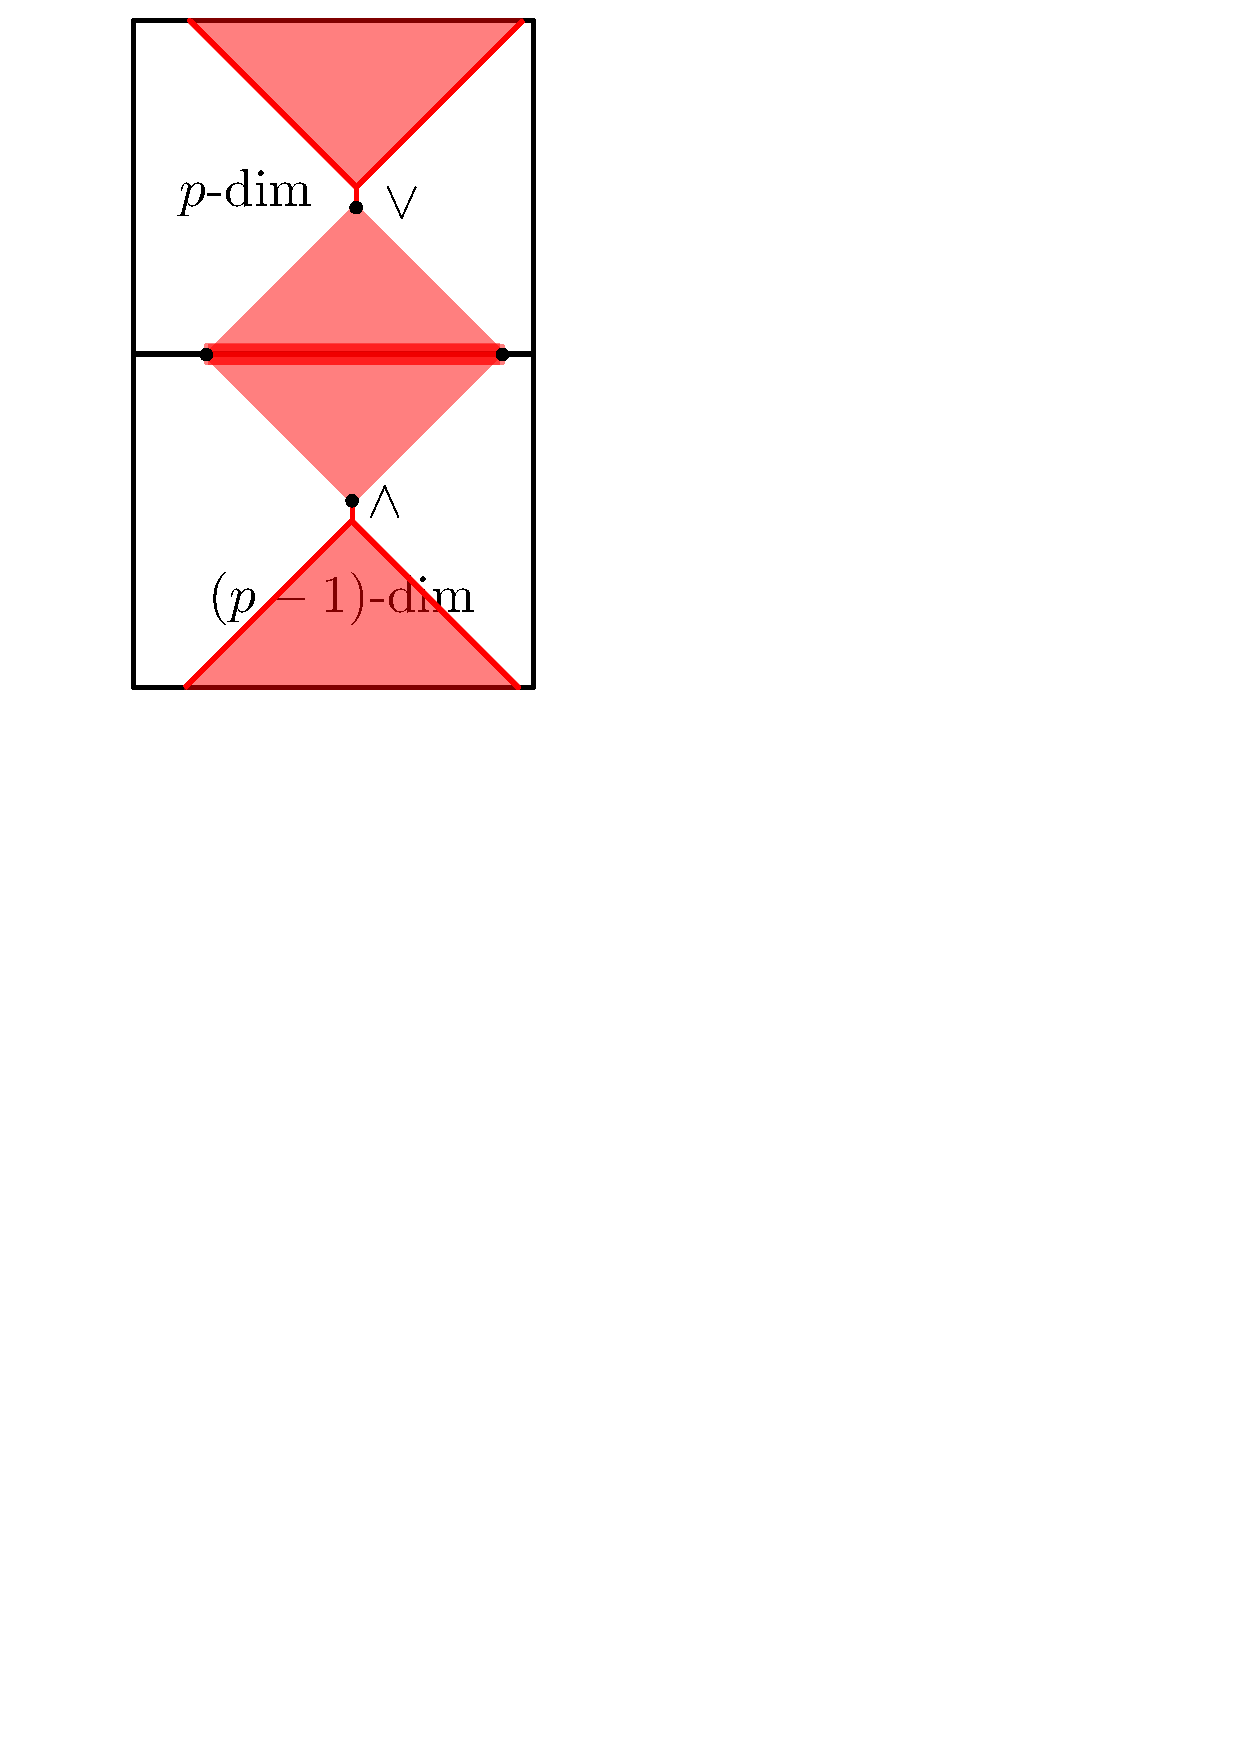
\includegraphics[height=5cm]{zigzag}
\caption{\label{fig:zz}  Here we show a possible choice of meet and
  join for  zig-zag persistence based on the M\" obius strip
  construction of~\cite{Car09}.}
\end{center}
\end{figure}

Using a special case of our construction, using pullbacks and pushouts as limits and colimits, the authors in~\cite{Sk12}, developed a parallelized algorithm for computing zig-zag persistence.  

To compare two general elements define
\begin{equation*}
\Hg_*(\X_i)\meet\Hg_*(\X_j) = \begin{cases} K \rto \Hg_*(\X_i)\oplus \Hg_*(\X_j)\rightrightarrows \Hg_*(\X_{i+1}) \qquad  j=i+2\\
\Hg_*(\X_i)\meet\Hg_*(\X_{i+2})\meet\cdots\meet\Hg_*(\X_j) \
\end{cases}
\end{equation*}
and
\begin{equation*}
\Hg_*(\X_i)\join\Hg_*(\X_j) = \begin{cases} \Hg_*(\X_{i+1}) \rightrightarrows  \Hg_*(\X_i)\oplus \Hg_*(\X_j) \rto P \qquad  j=i+2\\
\Hg_*(\X_i)\join\Hg_*(\X_{i+2})\join\cdots\join\Hg_*(\X_j) \
\end{cases}
\end{equation*}
With this definition it is not difficult to verify the following results
\begin{enumerate}
\item The rank of $\Hg_*(\X_i)\meet\Hg(\X_j)  \rightarrow
  \Hg_*(\X_i)\join\Hg(\X_j)$ is equal to the  rank in the original zig-zag
  definition.
\item The structure can be built up iteratively, comparing all
  elements two steps away then three steps away and
  so on, leading to the parallelized algorithm. 
\end{enumerate}
\begin{remark}
In \cite{Sk12}, an additional trick was used so that only the meets had to
be computed. 
\end{remark}


%%%%%%%%%%%%%%%%%%%%%%%%%%%%%%%%%%%%%%%%%


\subsection{Largest Injective}

%\begin{figure}
%\begin{center}
%\begin{tikzpicture}[very thick]
%\node (a) at (0,0) {$\X_0$};
%\node (b) at (0,2) {$\X_1$};
%\node (c) at (1,3) {$\X_2$};
%\node (d) at (2,0) {$\X_3$};
%\node (e) at (2,2) {$\X_4$};
%\node (f) at (3,-1) {$\X_5$};
%\node (g) at (4,0) {$\X_6$};
%\node (i) at (3,3) {$\X_7$};
%\node (h) at (4,2) {$\X_8$};
%\draw[->] (a) -- (b);
%\draw[->] (b) -- (c);
%\draw[->] (a) -- (e);
%\draw[->] (d) -- (e);
%\draw[->] (d) -- (b);
%\draw[->] (e) -- (c);
%
%\draw[->] (e) -- (i);
%\draw[->] (h) -- (i);
%\draw[->] (g) -- (h);
%\draw[->] (f) -- (g);
%\draw[->] (f) -- (d);
%
%\draw[->] (d) -- (h);
%
%\node (e1) at (1.5,-2) {\textcolor{red}{$\X_0 \wedge \X_5$}};
%\draw[->,red, dashed] (e1) -- (f) ;
%\draw[->,red, dashed] (e1) -- (a) ;
%
%\node (e2) at (2,4) {\textcolor{blue}{$\X_2 \vee \X_7$}};
%\draw[->,blue, dashed] (i) -- (e2) ;
%\draw[->,blue, dashed] (c) -- (e2) ;
%
%\end{tikzpicture}
%\end{center}
%
%\label{gendgm}
%\caption{The lattice completion of a general diagram.}
%\end{figure}

For the first application, we consider the computation of the largest injective of a diagram. 
In principle, we are looking for something which persists over an entire diagram. 
While satisfying the properties of the underlying lattice structure, the largest injective must fulfill to be in the following images 
%
\begin{equation*}
\im\left(\Hg_*(\X_i) \meet \Hg_*(\X_j) \rto \Hg_*(\X_i) \join
\Hg_*(\X_j)\right) \qquad \forall i,j
\end{equation*}
By completeness, it follows that this can be written as 
\begin{equation*}
\im \left(\bigwedge\limits_i \Hg_*(\X_j) \rto \bigvee\limits_i
\Hg_*(\X_i)\right) 
\end{equation*}
Using the order structure, we
can rewrite the above as
\begin{equation*}
\im \left(\bigwedge\limits_{i\in\mathrm{sources}} \Hg_*(\X_j) \rto \bigvee\limits_{j\in\mathrm{targets}}
\Hg_*(\X_j)\right). 
\end{equation*}
%
Recall that \emph{sources} are all the elements in original diagram which are not the codomain of any maps and \emph{targets} are the elements which are not the domain of any maps. 
%
Assuming we have $n$ sources, $m$ targets and the longest total order in the diagram is $k$ assuming an $O(1)$ time to compute a $\join$ or $\meet$ of two elements, we have a run time of $O(n+m+k)$. 
On a parallel machine, the operations can be computed independently and using associativity, we can construct the total meet/join using a binary tree scheme, giving a run time of $O(k+\log (\max(n,m)) )$.

\begin{center}

     \begin{tikzpicture}[scale=.7, thick] 

       \node (x1) at (1,1) {$\X_{1}$};
        \node (x2) at (3,1) {$\X_{2}$};
        \node (x3) at (5,1) {$\X_{3}$};
        
       \node (x4) at (1,-2) {$\X_{4}$};
        \node (x5) at (3,-2) {$\X_{5}$};
        \node (x6) at (5,-2) {$\X_{6}$};
        
        \draw[fill=black] (0,0) circle (0.05cm);
        \draw[fill=black] (2,0) circle (0.05cm);
        \draw[fill=black] (4,0) circle (0.05cm);
        \draw[fill=black] (6,0) circle (0.05cm);

        \draw[fill=black] (0,-1) circle (0.05cm);
        \draw[fill=black] (2,-1) circle (0.05cm);
        \draw[fill=black] (4,-1) circle (0.05cm);
        \draw[fill=black] (6,-1) circle (0.05cm);
        
        \draw[->] (0,0) edge (x1);
        \draw[->] (2,0) edge (x1);
        \draw[->] (2,0) edge (x2);
        \draw[->] (4,0) edge (x2);
        \draw[->] (4,0) edge (x3);
        \draw[->] (6,0) edge (x3);
        
        \draw[->] (x4) edge (0,-1);
        \draw[->] (x4) edge (2,-1);
        \draw[->] (x5) edge (2,-1);
        \draw[->] (x5) edge (4,-1);
        \draw[->] (x6) edge (4,-1);
        \draw[->] (x6) edge (6,-1);
        
        \node (x7) at (2,-3) {$\X_{7}$};
        \node (x8) at (4,-3) {$\X_{8}$};
        \node (x9) at (3,-4) {$\X_{9}$};

        \draw[->] (x7) edge (x4);
        \draw[->] (x7) edge (x5);
        \draw[->] (x8) edge (x5);
        \draw[->] (x8) edge (x6);
        \draw[->] (x9) edge (x7);
        \draw[->] (x9) edge (x8);       
        
        \node (x10) at (3,2) {$\X_{10}$};

        \draw[->, dashed] (x1) edge (x10);
        \draw[->, dashed] (x2) edge (x10);
        \draw[->, dashed] (x3) edge (x10);

     \end{tikzpicture}

\begin{equation*}
\im \left(\bigwedge\limits_{i\in\mathrm{sources}} \Hg_*(\X_j) \rto \bigvee\limits_{j\in\mathrm{targets}}\Hg_*(\X_j)\right) 
\end{equation*}

\end{center}


Unfortunately, we cannot always compute the meet or join in constant time as we may need to compose a linear number of maps. In the future, we will do a more fine grain analysis, but we note that given that we have a
distributive lattice, all maximal total orders are of constant length, allowing us to bound the time to compute any meet and join by this length. 



%%%%%%%%%%%%%%%%%%%%%%%%%%%%%%

\subsection{Sections}

Finally we return to the bifiltration case to highlight the difference between our construction and the one we presented in Section~\ref{Problem Statement} which yielded the rank invariant. 
Consider Figure~\ref{fig:sections}. The rank invariant requires that all the elements of a square have class to contribute to the rank of the square. 
However, using our construction, a class will persist between two elements if and only if there is a sequence of maps in the diagram such that the classes map into each other (or from each other). 
In this case we can find persistent sections across incomparable elements yielding finer grained information than the rank invariant.
Furthermore, in highly structured diagrams such as multifiltrations, additional properties such as associativity have algorithmic consequences as well. 

\begin{figure}%[ht]
%
\subfigure[sections]{
%
     \begin{tikzpicture}[thick, scale=0.6] 
         \foreach \i  [evaluate=\i as \x using int(2*\i)] in {0,...,3}{
           \foreach \j [evaluate=\j as \y using int(2*\j)] in {0,...,3}{
             \node (p\i\j) at (\x,\y) {$\X_{\i\j}$}    ;
           }
         }
         \foreach \i [evaluate=\i as \x using int(\i+1)] in {0,...,2}{
           \foreach \j [evaluate=\j as \y using int(\j+1)]  in {0,...,2}{
             \draw[->] (p\i\j) -- (p\i\y)  ;
             \draw[->] (p\i\j) -- (p\x\j)  ;
           }
         }

         \foreach \j [evaluate=\j as \y using int(\j+1)]  in {0,...,2}{
           \draw[->] (p3\j) -- (p3\y)  ;
           \draw[->] (p\j3) -- (p\y3)  ;
           }
%                   
         \node (j1) at (2.5,2.5) {$\wedge$};
         \node (m1) at (3.5,3.5) {$\vee$};         
         \draw[->,dashed, red] (j1) -- (p12) ;
         \draw[->,dashed, red] (j1) -- (p21) ;
         \draw[->,dashed, red] (p12) -- (m1) ;
         \draw[->,dashed, red] (p21) -- (m1) ;
%
         \node (j) at (0.5,4.5) {$\wedge$};
         \node (m) at (1.5,5.5) {$\vee$};         
         \draw[->,dashed, red] (j) -- (p03) ;
         \draw[->,dashed, red] (j) -- (p12) ;
         \draw[->,dashed, red] (p12) -- (m) ;
         \draw[->,dashed, red] (p03) -- (m) ;
%
         \node (j2) at (4.5,0.5) {$\wedge$};
         \node (m2) at (5.5,1.5) {$\vee$};         
%
         \draw[->,dashed, red] (j2) -- (p30) ;
         \draw[->,dashed, red] (j2) -- (p21) ;
         \draw[->,dashed, red] (p30) -- (m2) ;
         \draw[->,dashed, red] (p21) -- (m2) ;
%
     \end{tikzpicture}
% 
\label{exsections2}
}
%
% 
\subfigure[associativity]{
%
     \begin{tikzpicture}[thick, scale=0.6]
         \foreach \i  [evaluate=\i as \x using int(2*\i)] in {0,...,3}{
           \foreach \j [evaluate=\j as \y using int(2*\j)] in {0,...,3}{
             \node (p\i\j) at (\x,\y) {$\X_{\i\j}$}    ;
           }
         }
         \foreach \i [evaluate=\i as \x using int(\i+1)] in {0,...,2}{
           \foreach \j [evaluate=\j as \y using int(\j+1)]  in {0,...,2}{
             \draw[->] (p\i\j) -- (p\i\y)  ;
             \draw[->] (p\i\j) -- (p\x\j)  ;
           }
         }
%
         \foreach \j [evaluate=\j as \y using int(\j+1)]  in {0,...,2}{
           \draw[->] (p3\j) -- (p3\y)  ;
           \draw[->] (p\j3) -- (p\y3)  ;
           }
%        
         \node (j1) at (2.5,2.5) {$\wedge$};
         \node (m1) at (3.5,3.5) {$\vee$};         
         \draw[->,dashed, red] (j1) -- (p12) ;
         \draw[->,dashed, red] (j1) -- (p21) ;
         \draw[->,dashed, red] (p12) -- (m1) ;
         \draw[->,dashed, red] (p21) -- (m1) ;
%
         \node (j) at (0.5,4.5) {$\wedge$};
         \node (m) at (1.5,5.5) {$\vee$};         
         \draw[->,dashed, red] (j) -- (p03) ;
         \draw[->,dashed, red] (j) -- (p12) ;
         \draw[->,dashed, red] (p12) -- (m) ;
         \draw[->,dashed, red] (p03) -- (m) ;
%
         \node (j2) at (0.5,2.5) {$\wedge$};
         \node (m2) at (3.5,5.5) {$\vee$};         
%
         \draw[->,dashed, red] (j2) -- (j) ;
         \draw[->,dashed, red] (j2) -- (j1) ;
         \draw[->,dashed, red] (m1) -- (m2) ;
         \draw[->,dashed, red] (m) -- (m2) ;
%
     \end{tikzpicture}
%     
\label{exsections1}
}
\caption{\label{fig:sections}
While the associativity of the lattice operations in the bifiltration corresponds to the possible paths in the diagram \subref{exsections1}, the sections in the lattice can be explained by the diagram \subref{exsections2}.
}
\label{exsections}
\end{figure}






%%%%%%%%%%%%%%%%%%%%%%%%%%%%%%%%%%%%%%%%%%%%%%
%%%%%%%%%%%%%%%%%%%%%%%%%%%%%%%%%%%%%%%%%%%%%%


\section{Discussion}
\label{discussion}


In this paper, we have investigated the properties of a lattice which contains information about the persistent homology classes in a general commutative diagram of vector spaces. There are still numerous open questions including:
\begin{itemize}
\item What kind of decompositions exist in the spirit of persistence diagrams for this distributive lattice, since all maximal total orders are the same length and therefore we can decompose this lattice into a canonical sequence of antichains?
\item What are further algorithmic implications of this structure?
\item What is the correct metric to consider to general commutative diagrams as ``close''?
\item In what other contexts do such diagrams appear and what can we say about their structure?
\end{itemize}
We will address some of these questions in a subsequent paper. 



%%%%%%% BIBLIOGRAPHY %%%%%%%%%%%%%%%%%%%%%%%%%%%%%%%%
						
\bibliographystyle{plain}

\begin{thebibliography}{10}

\bibitem{CatCS}
M. Barr and C. Wells.
\newblock {\em Category theory for computing science}, volume~10.
\newblock Prentice Hall, 1990.

\bibitem{Ba13}
A. Bauer, K. Cvetko-Vah, M. Gehrke, S. J. van Gool, and G. Kudryavtseva.
\newblock A non-commutative Priestley duality.
\newblock {\em Topology and its Applications}, 2013.

\bibitem{Be10}
G. Bezhanishvili.
\newblock Bitopological duality for distributive lattices and Heyting algebras.
\newblock {\em Mathematical Structures in Computer Science}, 20(3):359--393,
  2010.

\bibitem{Be06}
N. Bezhanishvili.
\newblock {\em Lattices of intermediate and cylindric modal logics.}
\newblock Institute for Logic, Language and Computation, 2006.

\bibitem{Ba40}
G. Birkhoff.
\newblock {\em Lattice theory}, volume~5.
\newblock AMS Colloquium Publications, Providence RI, third edition, 1940.

\bibitem{Bu14}
P. Bubenik and J. A. Scott.
\newblock {Categorification of persistent homology}.
\newblock In {\em Discrete \& Computational Geometry}, 51(3):600--627 2014.

\bibitem{Sa81}
S. Burris and H. P. Sankappanavar.
\newblock {\em A course in universal algebra}.
\newblock S. Burris and H. P. Sankappanavar, 1981.

\bibitem{TD}
G. Carlsson.
\newblock {Topology and data}.
\newblock {\em Bulletin-American Mathematical Society}, 46(2):1--54, 2009.

\bibitem{Car09}
G. Carlsson, V. De~Silva, and D. Morozov.
\newblock {Zigzag persistent homology and real-valued functions.}
\newblock In {\em Proceedings of the Annual Symposium on Computational
  Geometry}, pages 247--256, March 2009.

\bibitem{Carl09}
G. Carlsson and A. Zomorodian.
\newblock {The theory of multidimensional persistence}.
\newblock {\em Discrete {\&} Computational Geometry}, 42(1):71--93, 2009.

\bibitem{ZigZag}
G. Carlsson and V. de~Silva.
\newblock Zigzag persistence.
\newblock {\em Found. Comput. Math.}, 10(4):367--405, 2010.

\bibitem{Zom09}
G. Carlsson, G. Singh and A. Zomorodian.
\newblock {Computing Multidimensional Persistence}.
\newblock {\em arXiv.org}, July 2009.

\bibitem{Da02}
B. A. Davey and H. A. Priestley.
\newblock {\em Introduction to lattices and order.}
\newblock Cambridge University Press, 2002.

\bibitem{Dil50}
R. P. Dilworth.
\newblock A decomposition theorem for partially ordered sets.
\newblock {\em Annals of Mathematics}, 51(1):161--166, 1950.

\bibitem{Is08}
A. D\"{o}ring and C. Isham.
\newblock A topos foundation for theories of physics: I. formal languages for
  physics.
\newblock {\em Journal of Mathematical Physics}, 49, 2008.

\bibitem{Ed10}
H. Edelsbrunner and J. L. Harer.
\newblock {\em Computational Topology: An Introduction}.
\newblock American Mathematical Society, 2010.

\bibitem{Edel00}
H. Edelsbrunner, D. Letscher, and A. Zomorodian.
\newblock {Topological persistence and simplification}.
\newblock {\em Discrete {\&} Computational Geometry}, 28(4):511--533, December
  2012.

\bibitem{Fa96}
J. D. Farley.
\newblock The automorphism group of a function lattice: A problem of J\' onsson
  and McKenzie.
\newblock {\em Algebra Universalis}, 36(1):8--45, 1996.

\bibitem{Gr71}
G. Gr\"{a}tzer.
\newblock {\em Lattice theory}.
\newblock WH Freeman and Co, San Francisco, 1971.

\bibitem{Gr79}
G. Gr\"{a}tzer.
\newblock {\em Universal Algebra}.
\newblock Springer, second edition, 1979.

\bibitem{Hat00}
A. Hatcher.
\newblock {\em {Algebraic Topology}}.
\newblock Hatcher, December 2000.

\bibitem{Joh86}
P. T. Johnstone.
\newblock {\em {Stone Spaces}}.
\newblock Cambridge University Press, August 1986.

\bibitem{La87}
S. Lang.
\newblock {\em Linear Algebra}.
\newblock Springer, 3rd edition, 1987.

\bibitem{Lang}
S. Lang.
\newblock {\em Algebra}, volume 211.
\newblock Graduate texts in mathematics, 2002.

%\bibitem{Lu00}
%W. A. Luxemburg and A. C. Zaanen.
%\newblock {\em Riesz spaces}.
%\newblock North-Holland Publishing Company, 1971.

\bibitem{Le13}
J. Leech M. Kinyon and J. Pita Costa.
\newblock Distributive skew lattices.
\newblock {\em Submitted to Semigroup Forum}, 2013.

\bibitem{La98}
S. Mac~Lane.
\newblock {\em Categories for the Working Mathematician}.
\newblock Springer, 1998.

\bibitem{Mir71}
L. Mirsky.
\newblock A dual of Dilworth's decomposition theorem.
\newblock {\em American Mathematical Monthly}, 78(8):876--877, 1971.

\bibitem{Oud12}
S. Oudot and D. Sheehy.
\newblock {Zigzag Zoology: Rips Zigzags for Homology Inference}.
\newblock In {\em Proceedings of the twenty-ninth annual symposium on
  Computational geometry}, pages 387--396, 2012.

\bibitem{Be12}
H. Edelsbrunner P. Bendich, S. Cabello.
\newblock A point calculus for interlevel set homology.
\newblock {\em Pattern Recognition Letters}, 33(11):1436--1444, 2012.

\bibitem{Po05}
A. Polishchuk and L. Positselski.
\newblock {\em Quadratic Algebras, Clifford Algebras, and Arithmetic Witt
  Groups}.
\newblock American Mathematical Society, 2005.

\bibitem{Sk12}
P. {\v S}kraba and M. Vejdemo-Johansson.
\newblock Parallel and scalable zig-zag persistent homology.
\newblock In {\em NIPS 2012 Workshop on Algebraic Topology and Machine
  Learning.}, 2012.

\bibitem{Skr13}
P. {\v S}kraba and M. Vejdemo-Johansson.
\newblock {Persistence modules: Algebra and algorithms}.
\newblock {\em arXiv}, cs.CG, February 2013.

\bibitem{Tug98}
A. A. Tuganbaev.
\newblock {\em Semidistributive Modules and Rings}.
\newblock Mathematics and Its Applications. Springer, 1998.

\bibitem{Yo42}
K. Yosida.
\newblock On the representation of the vector lattice.
\newblock {\em Proceedings of the Japan Academy, Series A, Mathematical
  Sciences}, 18(7):339--342, 1942.

\bibitem{Zom13}
A. Zomorodian, G. Carlsson, A. Collins, and L. Guibas.
\newblock {Persistence Barcodes for Shapes}.
\newblock {\em International Journal of Shape Modeling (2oo5)}, pages 1--12,
  January 2013.

\bibitem{Zom05}
A. J. Zomorodian.
\newblock {\em {Topology for computing}}, volume~16.
\newblock Cambridge University Press, 2005.

\end{thebibliography}



%%%%%%%% THE END   :)  %%%%%%%%%%%%%%%%%%%%%%%%%%%%%%%%%

\end{document}
